\documentclass[border=10pt]{standalone}
\usepackage{amsfonts,amsmath,amssymb,amsthm}
\usepackage{tikz}
\usetikzlibrary{arrows.meta,shapes, calc}
\tikzset{%
  >={Latex[width=2mm,length=2mm]},
  % Specifications for style of nodes:
     base/.style = {rectangle, rounded corners, draw=black,
                           minimum width=4cm, minimum height=1.5cm,
                           text centered, font=\sffamily},
    stressUpdate/.style = {base, minimum width=2.5cm, fill=orange!15},
    newtonIteration/.style = {base, fill=blue!20},
    constitutiveModel/.style = {base, minimum width=2.5cm, fill=green!15},
    convergenceCheck/.style={newtonIteration, diamond, aspect=2},
}

\begin{document}    
  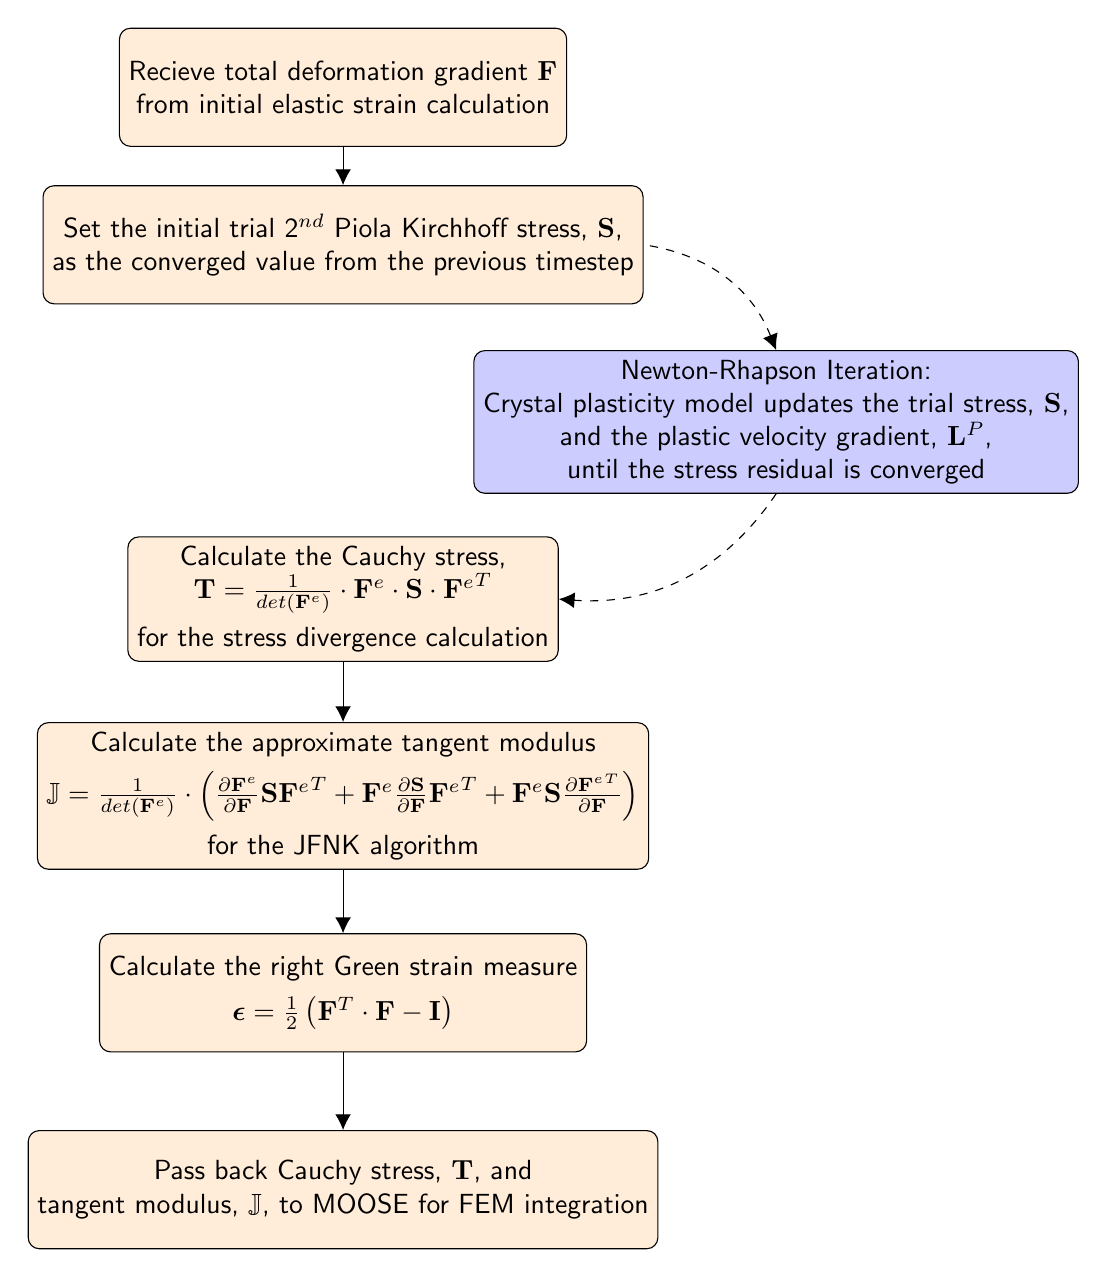
\begin{tikzpicture}[node distance=1.5cm,
    every node/.style={fill=white, font=\sffamily}, align=center]
  % Specification of nodes (position, etc.)
  \node (start)               [stressUpdate]
                              {Recieve total deformation gradient $\mathbf{F}$ \\ from initial elastic strain calculation};
  \node (trialStressBlock)    [stressUpdate, below of=start, yshift=-0.5cm]
                              {Set the initial trial 2$^{nd}$ Piola Kirchhoff stress, $\mathbf{S}$, \\ as the converged value from the previous timestep};
  \node (NewtonIterationBlock)  [newtonIteration, right of=trialStressBlock, xshift=4.0cm, yshift=-2.25cm]
                              {Newton-Rhapson Iteration: \\ 
                          Crystal plasticity model updates the trial stress, $\mathbf{S}$,\\
                               and the plastic velocity gradient, $\mathbf{L}^P$, \\
                               until the stress residual is converged};  
  \node (CauchyStressBlock)    [stressUpdate, below of=trialStressBlock, yshift=-3cm]
                              {Calculate the Cauchy stress, \\
                              $\mathbf{T} = \frac{1}{det\left( \mathbf{F}^e \right)} \cdot \mathbf{F}^e \cdot \mathbf{S} \cdot {\mathbf{F}^e}^T  $\\ [0.15cm]
                              for the stress divergence calculation};                            

  \node (tangentModulusBlock)    [stressUpdate, below of=CauchyStressBlock, yshift=-1cm] 
                              {Calculate the approximate tangent modulus \\ [0.15cm]
                              $\mathbb{J} = \frac{1}{det\left( \mathbf{F}^e \right)} \cdot \left( \frac{\partial \mathbf{F}^e}{\partial \mathbf{F}} \mathbf{S} {\mathbf{F}^e}^T + \mathbf{F}^e \frac{\partial \mathbf{S}}{\partial \mathbf{F}} {\mathbf{F}^e}^T + \mathbf{F}^e \mathbf{S} \frac{\partial {\mathbf{F}^e}^T}{\partial \mathbf{F}} \right) $ \\ [0.15cm]
                              for the JFNK algorithm};
                              
  \node (lagrangianBlock) [stressUpdate, below of=tangentModulusBlock, yshift=-1cm]
                              {Calculate the right Green strain measure \\[0.15cm]
                              $\boldsymbol{\epsilon} = \frac{1}{2}\left( \mathbf{F}^T \cdot \mathbf{F} - \mathbf{I} \right)$};
  \node (passBackBlock) [stressUpdate, below of=lagrangianBlock, yshift=-1cm] 
                              {Pass back Cauchy stress, $\mathbf{T}$, and \\
                              tangent modulus, $\mathbb{J}$, to MOOSE for FEM integration};


 
  % Specification of lines between nodes specified above
  % with aditional nodes for description 
  \draw[->]                   (start) to (trialStressBlock);

  \draw[<-, bend right=30, dashed] (NewtonIterationBlock.north) to (trialStressBlock.east);
  \draw[->, bend left=30, dashed]  (NewtonIterationBlock.south) to (CauchyStressBlock.east);
  
  \draw[->]        (CauchyStressBlock) to (tangentModulusBlock);
  \draw[->]        (tangentModulusBlock) to (lagrangianBlock);
  \draw[->]        (lagrangianBlock) to (passBackBlock);

  \end{tikzpicture}
\end{document}